
%(BEGIN_QUESTION)
% Copyright 2015, Tony R. Kuphaldt, released under the Creative Commons Attribution License (v 1.0)
% This means you may do almost anything with this work of mine, so long as you give me proper credit
\input preamble.tex

\begin{center}
\vskip 5pt 
\textbf{Reguleringstkenikk -- Nivå 2 }
\vskip 5pt 
\textbf{Arbidsoppdrag på Stasjon 3/4}
\vskip 5pt 
\textbf{Nivå- og Flow regulering}
\end{center}


I dette arbeidsoppdraget skal du sette i drift nivåregulering på en stasjon. Du skal prøve optimalisere PID parametrene på følgende måter\begin{itemize}[noitemsep]
\item Z\&N svingemetode
\item Skogestads metode
\end{itemize}
I dette arbeidsoppdraget skal du sette i drift strømningsregulering på en stasjon. Du skal prøve optimalisere PID parametrene på følgende måter\begin{itemize}[noitemsep]
\item Z\&N svingemetode
\item Skogestads metode
\item Lærerens jukse metode
\end{itemize}



%$$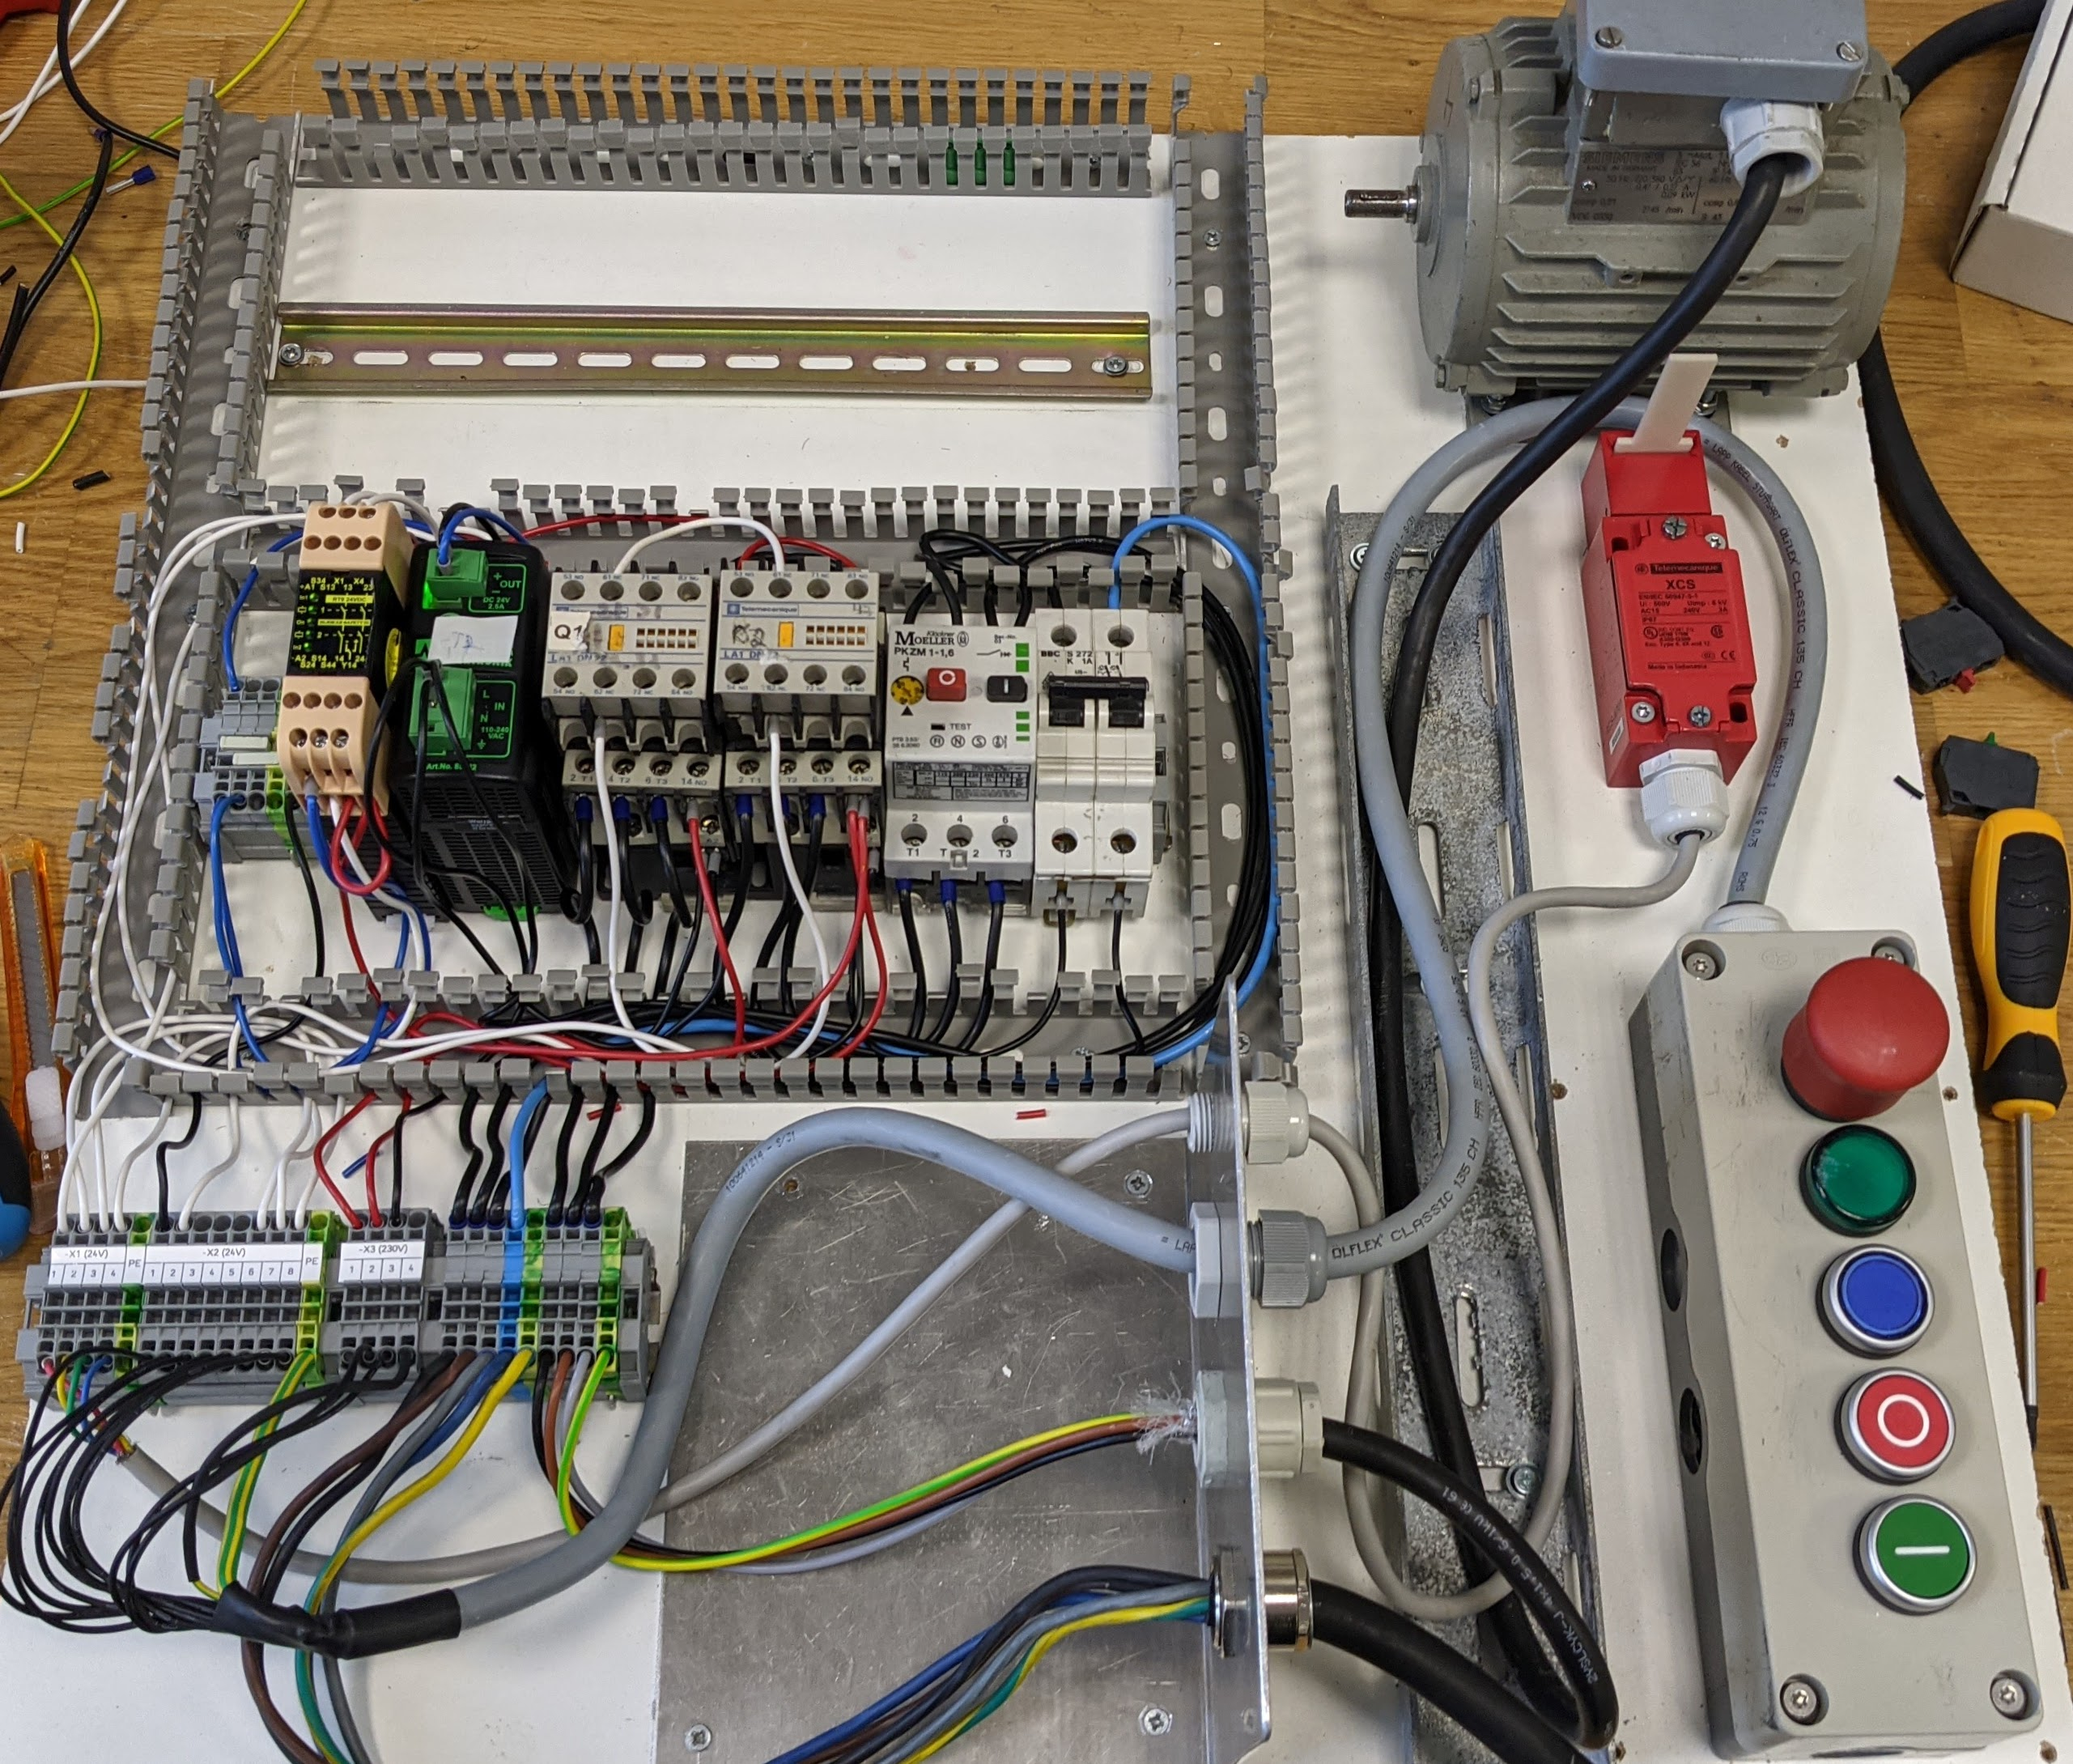
\includegraphics[width=13cm]{i04821x01.jpg}$$\\
\textbf{Teorioppgaver}

\textbf{Planlegging}

\textbf{Gjennomføring}

\textbf{Dokumentasjon}

Lag et dokument som viser hvordan du gikk frem for å optimalisere med de ulike metodene. 

\vskip 5pt
\begin{center}
\textbf{Arbidsoppdrag}
\vskip 5pt 
\textbf{Programmering av reguleringsstasjon}
\end{center}

\vskip 10pt 
\textbf{Introdusjon}

\vskip 5pt 

\vskip 5pt 

%$$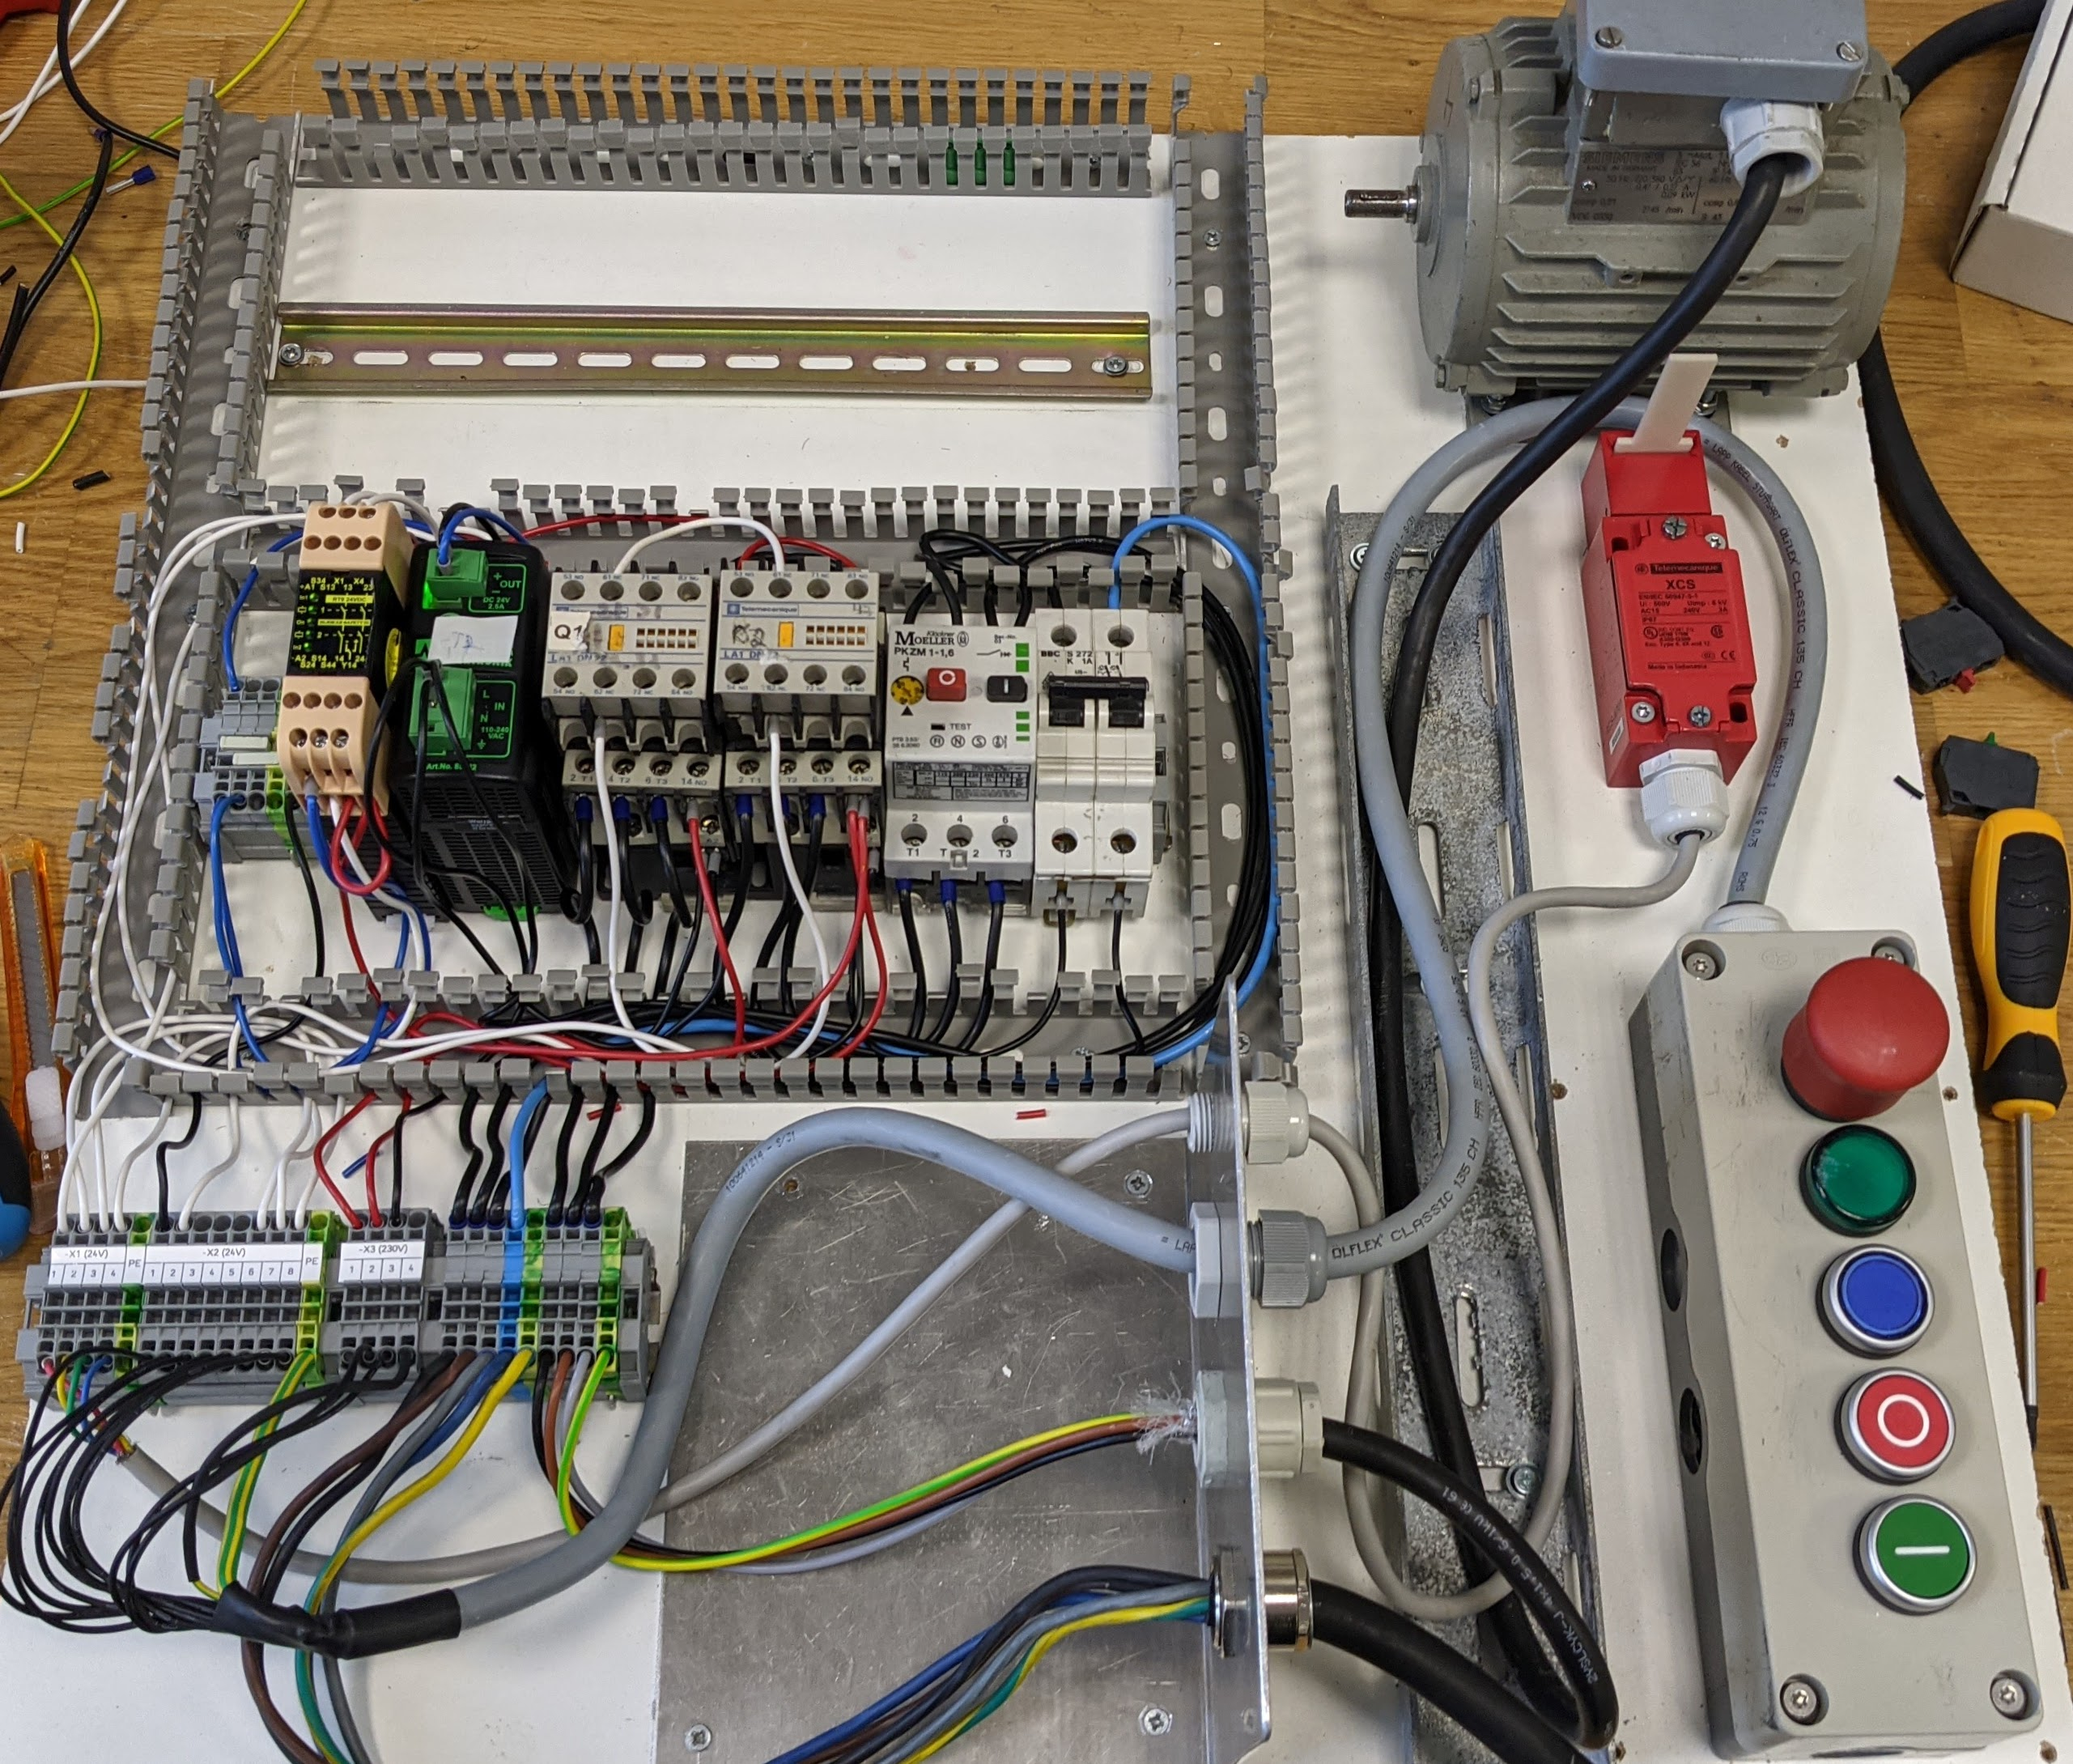
\includegraphics[width=13cm]{i04821x01.jpg}$$\\

\vskip 10pt 
\textbf{Teorioppgaver}

\vskip 5pt 

\vskip 10pt 
\textbf{Planlegging}


\vskip 10pt 
\textbf{Gjennomføring}

\vskip 10pt 
\textbf{Dokumentasjon}

Beskriv hvordan du planlegger, gjennomfører og dokumenterer denne jobben. 

















\end{document}
